Our app will be mobile based app that can run both on android as well as ios operating system. We are going to implement a simple user interface where a user can interact and perform all necessary tasks within the app with ease. Basically, at high level our user wants to store something safely where he won't forget. We help user do just that with the help of our app. First, We let the user to define the area where he would like to store his item. Then we let him store the item in the storage and then we will record the information about the item in the database, and retrieve it when it is needed. User will be able to use his camera for scanning the item, he does not have to manually enter every detail about the item that he wants to store. Similarly, once the user scans the picture of the item we will store items information in the database with its specific information. When he wants to retrieve the item he can simply search for the item in the app and the app will tell him where he stored the item, when and what are the important information about the item that he needs to know. for example the item is something that expires, the app will tell the user that it is going to expire on this date once searched. Also, if something is not searched and its expiry date is near then also the app will automatically notify the user about its expiry date. 
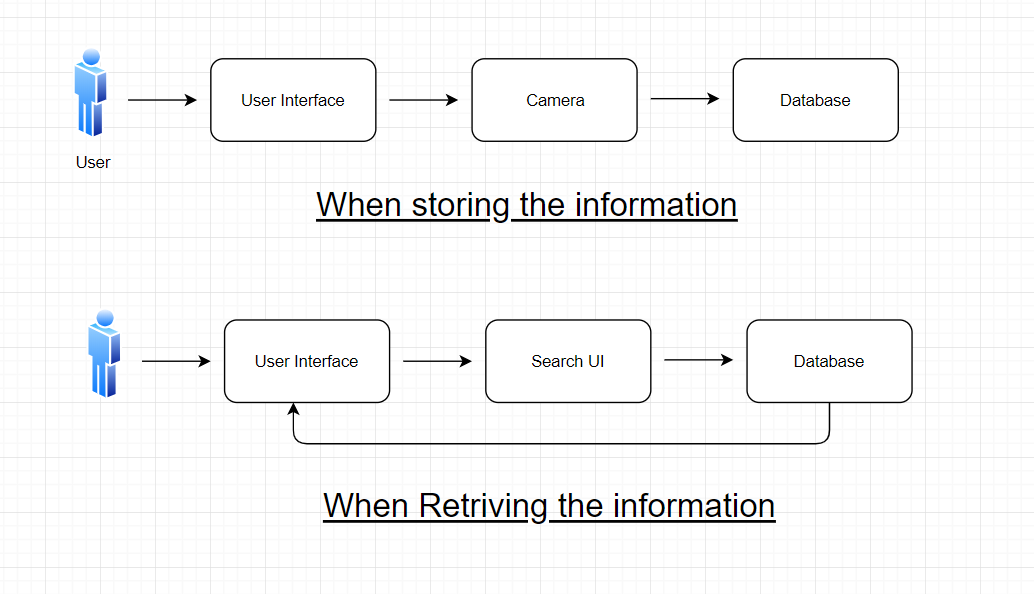
\includegraphics{project charter latex/images/component.PNG}